\chapter{Problem Definition and Algorithm Definition}

In this chapter, we'll take a close look at the core algorithm of \textit{MLANN} method. The next is dedicated to the implementation procedure of the algorithm.

\subsection{MLANN; General Idea} 
Despite the most of known fast approximate NN algorithms, the proposed method is not heuristic. The joint probabilistic densities (likelihoods) of the distances to previously checked reference objects are estimated for each class. The next reference instance is selected from the class with the maximal likelihood. To deal with the quadratic memory requirement of this approach, the author has proposed its modification, which processes the distances from all instances to a small set of pivots chosen with the farthest-first traversal. Experimental study in face recognition with the histograms of oriented gradients and the deep neural network-based image features shows that the proposed method is much faster than the known approximate NN algorithms for medium databases \cite{def1}.

\subsection{How Statistical Face Recognition Works}
In face recognition, we are required to assign an observed image $X$ to one of $R$ classes which is specified by the database of reference images. In this method, feature maps extracted from observed and reference images are treated as probability distributions. The following subsection provides baseline assumptions for this task.

\subsubsection{Key Assumptions}
In face recognition task with statistical method, we assume that
\begin{enumerate}
	\item The reference images from different classes are independent;
	\item The probability distributions of the feature vectors from the same class are identical \cite{def1}.
\end{enumerate}

\subsection{Where the Problem Arises}
The core algorithm of many face recognition implementations use \textit{Nearest Neighbor} method as the main approach to find the most similarity between the input image and the reference images in the database. Let $X$ be the observed image and $X_r \ r\in{1, ... R}$ be each of the images in the reference database. In that case, the optimal maximal likelihood solution of the face recognition task is achieved by
\begin{equation}
	W_v: v = arg\min\limits_{r}\ \rho(X, X_r)
\end{equation}
where $r$ is selected in a \textit{brute-force} manner by the nearest neighbor algorithm and $\rho$ is mean to be the \textit{distance} of two image feature maps.

\subsection{Speeding up the Search Process}
\subsubsection{Approximate Nearest Neighbor}
To speed-up the search process, we can use \textit{approximate} techniques. As an example, an approximate method is provided in \cite{def2}. This method is based on the following criterion:
\begin{equation}
	W_v: \rho(X, X_v) < \rho_0
\end{equation}
which is the termination condition of the \textit{ANN} method with respect to a bound of of $\rho_0$.

\subsubsection{Best-Bin First kd-tree}
In this method, the first reference image $X_{r_1},\ r_1 \in \{1, ... , R\}$ is randomly chosen. Next, it is put into the priority queue if reference images sorted by the distance to $X$. Next, the highest priority item $X_i$ is pulled from the queue and the set of reference images $X_i^{(M)}$ is determined by using the following expression:
\begin{equation}
	(\forall X_k \in X_i^{(M)})(\forall X_j \notin X_i^{(M)})|\rho_{i, k} - \rho(X, X_k)| \leq |\rho_{i, j} - \rho(X, X_j)|
\end{equation}
the distance matrix $P = [\rho_{i, j}]$ is computed at the beginning of the algorithm.


\subsubsection{Maximum Likelihood Approximate Nearest Neighbor Method}
Here is the core algorithm of this paper. The method is proposed for the next step reference image choice. Let the reference images $X_{r_1}, ..., X_{r_k}$ have been checked before the $k$-th step, meaning that the distances\\ $\rho(X, X_{r_1}), \rho(X, X_{r_2}), ...\rho(X, X_{r_k})$ have been computed. We can choose the next most probable reference image $X_{r_{k+1}}$ as
\begin{equation}
	r_{k + 1} = argmax (p_v . \prod_{i = 1}^{k}f(\rho(X, X_{r_i}) | W_v)) \ \ v\in\{1, ... R\} - \{r_1, ... r_k\}
\end{equation}
where $p_v$ is the prior probability of class $v$ which is the class of the observed image. $f(\rho(X, X_{r_i}) | W_v)$ is the conditional density of the distance $\rho(X, X_{r_i})$ if the hypothesis $W_v$ is true. We can acquire the likelihood $f(\rho(X, X_{r_i}) | W_v)$ using a \textit{Homogeneity Testing Probabilistic Neural Network}. Using an small modification proposed in the paper, we can obtain
\begin{equation}
	r_{k + 1} = argmin(\sum_{i = 1}^{k}\phi_\mu(r_i) - \ln p_\mu) \ \ \mu \in \{1, ... R\} - \{r_1, ... r_k\}
\end{equation}
where $\phi_\mu(r_i)$ satisfies all we need for a normal distribution:
\begin{equation}
	\phi_\mu(r_i) = \frac{(\rho(X, X_{r_i}) - \rho_{\mu, r_i} - \frac{N - 1}{UV}))^2}{\rho_{\mu, r_i}} + \frac{4}{UV}\ln (2\rho_{\mu, r_i} + \frac{N - 1}{UV})
\end{equation}
since the average image size is usually much higher than the number of parameters $UV >> (N - 1)$, $\phi_\mu(r_i)$ can be simplified:
\begin{equation}
	\phi_\mu(r_i) = \frac{(\rho(X, X_{r_i}) - \rho_{\mu, r_i}))^2}{\rho_{\mu, r_i}}
\end{equation}
If the distance $\rho(X, X_{r_{k + 1}})$ is lower than the threshold $\rho_0$, then the search procedure is terminated at the $K_{checks} = k + 1$ step. Otherwise, the reference image $X_{r_{k + 1}}$ is put into the set of previously checked reference images and the maximal likelihood search procedure is repeated.

\subsection{MLANN; Disadvantages}
Though the proposed MLANN method makes it possible to minimize the average number of distance computations $K_{checks}$, it has two significant disadvantages:
\begin{itemize}
	\item The necessity to compute and store distances between all reference images makes MLANN to use \textit{quadratic memory space}.
	
	\item The complexity of extra computation at each step is rather high. For instance, $\phi_\mu(r_i)$ is calculated for each unchecked $\mu$-th reference image.
\end{itemize}

\subsection{Pivot Based MLANN; An Improvement to MLANN Method}
In this section a modified version of MLANN is proposed. We'll choose $p << R$ reference images (pivots) from the database. The results show that the performance increases if we choose images far from each other. Thus it is necessary to choose the pivots as distant as possible. This task can be solved using known \textit{clustering} algorithms. Another approach is the incremental selection of pivots which is better compared to the clustering techniques which requires calculating the distances between all the images in database. We'll use the \textit{farthest-first traversal} procedure. The first pivot $X_{r_1}$ is chosen randomly. Next, the distances between this reference image and all other reference images are computed, and the most distant reference image is selected as the second pivot. The procedure is repeated so that every pivot is characterized with the highest sum of distances to the previous pivots:
\begin{equation}
	r_{i + 1} = argmax \sum_{j = 1}^{i}\rho(X_\mu, X_{r_j}), i \in \{1, ..., p - 1\}
\end{equation}
where 
$$
\mu \in \{1, ... R\} - \{r_1, ... r_i\}
$$
The result of the initialization phase is a list of pivots and $R * p$ matrix of distances between all reference images and the pivots.

\subsection{Time and Space Complexity Analysis}
Figure 2.1 demonstrates the time and space complexities of \textit{P-ML-ANN} method.
\begin{figure}[!h]\centering
	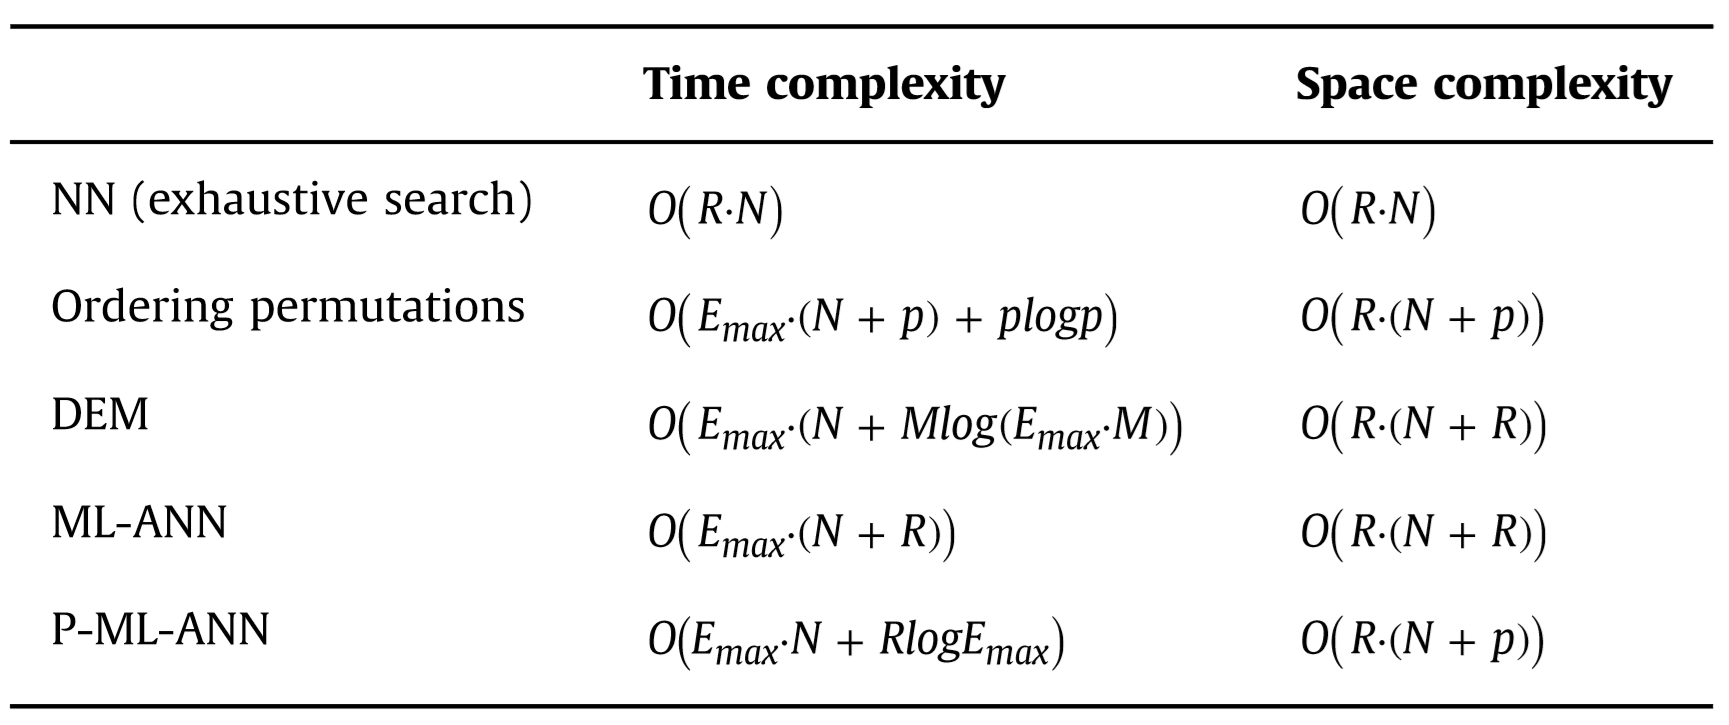
\includegraphics[width=0.8\textwidth]{complexities.PNG}
	\caption{Time and space complexities of the P-ML-ANN algorithm.}
	\label{pl1}
\end{figure}

